\documentclass{article}
\usepackage[usenames]{color} %used for font color
\usepackage{amsfonts}
\usepackage{amsmath}
\usepackage{amssymb}
\usepackage{array}
% \usepackage{amsthm}
\usepackage{bm}
\usepackage{bbm}
\usepackage{booktabs}
\usepackage{cite}
\usepackage{CJKutf8}
\usepackage{color}
\usepackage{comment}
\usepackage{courier}
\usepackage{enumerate}
\usepackage{enumitem}
\usepackage{epsfig}
\usepackage{eurosym}
\usepackage{float}
\usepackage[stable]{footmisc}
% \usepackage[bottom]{footmisc}
\usepackage[top=2.5cm,bottom=2.5cm,left=2.5cm,right=2.5cm]{geometry}
\usepackage{graphicx}  
\usepackage{helvet}
\usepackage{hhline}
\usepackage{hyperref}
\usepackage{imakeidx} % allows index generation
\usepackage{latexsym}
\usepackage{mathdots}
\usepackage{mathptmx}
\usepackage{microtype}
\usepackage{multicol}
\usepackage{multirow}
\usepackage{palatino}
\usepackage{pgfplots}
\pgfplotsset{compat=newest}
\usepackage{pdfsync}
\usepackage{psfrag}
\usepackage{pstricks}
\usepackage{subfigure}
\usepackage[many]{tcolorbox}
\usepackage{tikz,pgf}
\usetikzlibrary{backgrounds}
\usetikzlibrary{plotmarks}
\usepackage{tikz-layers}
\usepackage{type1cm}
\usepackage{ulem}
\usepackage{yfonts}


\def\x{\mathbf{x}}


\def\y{\mathbf{y}}
\def\c{\mathbf{c}}
\def\d{\mathbf{d}}
\def\A{\mathbf{A}}
\def\B{\mathbf{B}}
\def\b{\mathbf{b}}
\def\y{\mathbf{y}}
\def\Re{\mathbb{R}}
\def\Z{\mathbb{Z}}


\title{ISyE 6669 HW 13}
\date{Fall 2025}
\begin{document}
\maketitle

\begin{enumerate}
    \item Write linear constraints with continuous and integer variables for the following problems. You need to clearly define the variables that you introduce and give an explanation of your constraints.
    \begin{enumerate}
        \item If we invest \$50 or more on project 1, then we can only invest at most \$100 on project 2. Suppose the investment amount on each project is a continuous variable.
        
        \textbf{Solution:}
        
        Let $x_1$ and $x_2$ be continuous variables representing the investment amounts on project 1 and project 2, respectively. Let $\delta \in \{0,1\}$ be a binary variable and let $\varepsilon > 0$ be a very small constant. We assume that the possible values of $x_1$ and $x_2$ lie in some bounded region, and define
        \[
            M_1 := \max (x_1 - 50), \qquad
            M_2 := \max (x_2 - 100),
        \]
        over that region, so that $M_1 \ge 0$ and $M_2 \ge 0$.
        
        We model the if-then statement ``If $x_1 \geq 50$, then $x_2 \leq 100$'' by:
        \begin{align*}
            x_1 + \varepsilon &\leq 50 + \delta (M_1 + \varepsilon), \\
            x_2 &\leq 100 + M_2 (1 - \delta), \\
            \delta &\in \{0, 1\}.
        \end{align*}
        
        \textbf{Explanation:}
        \begin{itemize}
            \item If $\delta = 0$, the first constraint gives $x_1 + \varepsilon \leq 50$, i.e., $x_1 \leq 50 - \varepsilon < 50$, which is precisely the contrapositive statement ``if $\delta = 0$ then $x_1 < 50$''. The second constraint becomes $x_2 \leq 100 + M_2$, which is nonbinding because $M_2$ is chosen as an upper bound for $x_2 - 100$.
            \item If $\delta = 1$, the first constraint becomes $x_1 + \varepsilon \leq 50 + M_1$, which is automatically satisfied for all admissible $x_1$ (since by definition $x_1 - 50 \le M_1$ on the bounded region), while the second constraint reduces to $x_2 \leq 100$, enforcing the ``then'' part whenever $x_1 \ge 50$.
            \item The small positive constant $\varepsilon$ is used to handle the strict inequality in the contrapositive: instead of $x_1 < 50$ we impose $x_1 \le 50 - \varepsilon$, where $\varepsilon > 0$ is chosen sufficiently small compared with the scale of $x_1$. This yields a closed polyhedron that is equivalent for optimization purposes, while faithfully representing the intended logical condition.
        \end{itemize}
        The definitions $M_1 := \max(x_1 - 50)$ and $M_2 := \max(x_2 - 100)$ are taken over the bounded region of admissible $(x_1,x_2)$. With these choices we have
        \[
            x_1 - 50 \le M_1, \qquad x_2 - 100 \le M_2
        \]
        for all feasible $(x_1,x_2)$. Hence when $\delta = 1$, the first constraint $x_1 + \varepsilon \le 50 + (M_1+\varepsilon)$ is always satisfied and does not restrict $x_1$, while the second constraint tightens to $x_2 \le 100$. When $\delta = 0$, the first constraint enforces $x_1 < 50$ and the second becomes $x_2 \le 100 + M_2$, which is automatically satisfied and therefore nonbinding. In this way $M_1$ and $M_2$ are genuine Big-$M$ upper bounds chosen from the domain of $(x_1,x_2)$ so that the constraints relax in exactly the situations where the implication should not impose restrictions.
        
        \item If two continuous variables $x_1, x_2$ satisfy the linear constraint $x_1 + x_2 < 1$, then they also need to satisfy $x_1 - x_2 \ge 1$. Plot the feasible region of $(x_1, x_2)$ that satisfies the above if-then statement. Is this feasible region a convex set? Now use linear constraints with continuous and integer variables to model this if-then statement. Define all the variables you need and explain the constraints that you write down.
        
        \textbf{Solution:}
        
        The logical statement is
        \[
            (x_1 + x_2 < 1) \;\Rightarrow\; (x_1 - x_2 \ge 1).
        \]
        This is equivalent to saying that any feasible point must satisfy
        \[
            x_1 + x_2 \ge 1 \quad \text{or} \quad \bigl(x_1 + x_2 < 1 \;\text{and}\; x_1 - x_2 \ge 1\bigr).
        \]
        Hence the feasible region is the union of the halfspace $\{(x_1,x_2): x_1 + x_2 \ge 1\}$ and the region $\{(x_1,x_2): x_1 + x_2 < 1,\; x_1 - x_2 \ge 1\}$. This union is an "L-shaped" region (as in the provided plot) and is therefore \emph{not} convex, since we can find two feasible points whose midpoint does not belong to the feasible region.
        
        \begin{figure}[H]
        \centering
        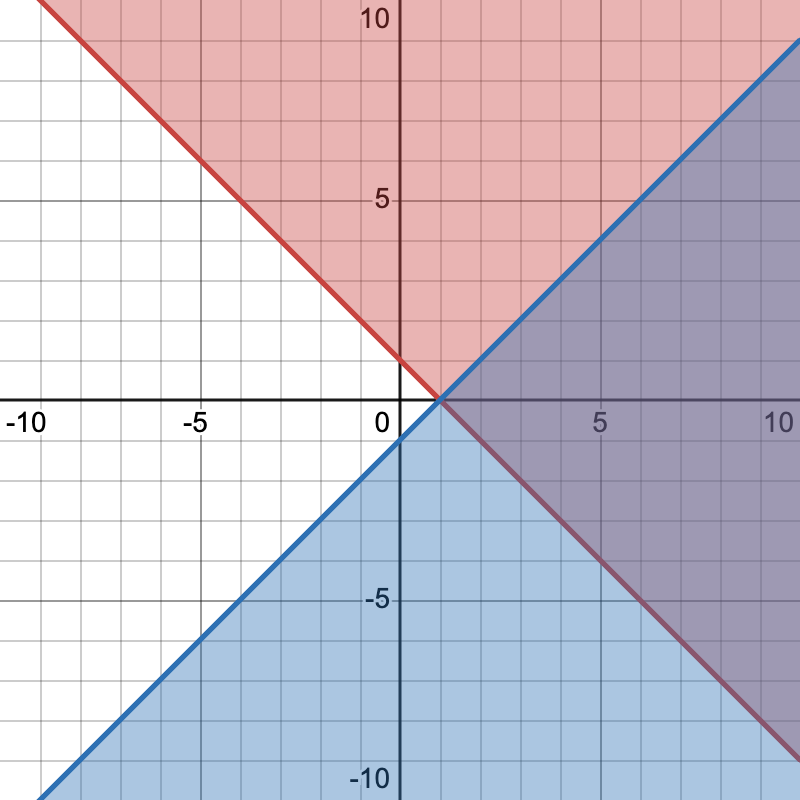
\includegraphics[width=0.6\textwidth]{HW13-1.png}
        \caption{Feasible region for the if-then statement $(x_1 + x_2 < 1) \Rightarrow (x_1 - x_2 \ge 1)$.}
        \end{figure}
        
        To model this if-then statement using linear constraints and a binary variable, let $x_1, x_2$ be continuous variables and let $\delta \in \{0,1\}$ be a binary variable. Define constants
        \[
            m_1 := \min (x_1 + x_2 - 1), \qquad
            m_2 := \min (x_1 - x_2 - 1),
        \]
        taken over the (bounded) region in which $(x_1,x_2)$ are allowed to vary. Note that $m_1 \le 0$ and $m_2 \le 0$. We then impose
        \begin{align*}
            x_1 + x_2 &\ge 1 + \delta\, m_1, \\
            x_1 - x_2 &\ge 1 + (1-\delta)\, m_2, \\
            \delta &\in \{0,1\}.
        \end{align*}
        
        \textbf{Explanation:}
        \begin{itemize}
            \item If $\delta = 0$, the first constraint gives $x_1 + x_2 \ge 1$, while the second becomes $x_1 - x_2 \ge 1 + m_2$. By the definition of $m_2$ this second inequality is automatically satisfied for all admissible $(x_1,x_2)$ and is thus nonbinding. This corresponds to the case where the “if” part is false, so we only need $x_1 + x_2 \ge 1$.
            \item If $\delta = 1$, the first constraint reduces to $x_1 + x_2 \ge 1 + m_1$, which is automatically satisfied by all admissible $(x_1,x_2)$, while the second constraint becomes $x_1 - x_2 \ge 1$, enforcing the “then” part when the “if” part holds.
        \end{itemize}
        The use of $\min$ in the definitions of $m_1$ and $m_2$ guarantees $m_1 \le 0$ and $m_2 \le 0$. Thus, when $\delta = 1$, the first constraint becomes $x_1 + x_2 \ge 1 + m_1 \le 1$, which is automatically satisfied by any point that already satisfies $x_1 + x_2 < 1$, and plays no restrictive role; only $x_1 - x_2 \ge 1$ remains active. When $\delta = 0$, the second constraint becomes $x_1 - x_2 \ge 1 + m_2 \le 1$, which is automatically satisfied, while $x_1 + x_2 \ge 1$ is enforced. In this way, $m_1$ and $m_2$ act as ``small-$m$'' parameters chosen from the domain of $(x_1,x_2)$ so that the constraints relax exactly in the branch where the implication is not binding.
        Therefore, the feasible $(x_1,x_2)$ for which there exists some $\delta \in \{0,1\}$ satisfying the above constraints are exactly those satisfying the original if-then statement.
        
    \end{enumerate}
    
    \item Suppose that you are interested in choosing a set of
investments $\{1, \dots, 7\}$. Assume that the investments have cost of
\$5, \$7, \$6, \$3, \$9, \$12, \$5. Assume there is a budget of \$30.
Also assume that the eventual expected profit out of each
investment is \$1, \$3, \$2, \$4, \$1, \$5, \$4. Write an optimization model to maximize profit with the following constraints. The objective function and all the constraints should be linear and there may be integer variables. Define all variables you need and explain the constraints that you write down.
\begin{enumerate}
\item You must choose at least one of the investments.
\item Investment 1 cannot be chosen if investment 3 is chosen.
\item Investment 4 can be chosen only if investment 2 is also
chosen.
\item You must choose either both investments 1 and 5 or
neither.
\item You must choose either at least one of the investments
1, 2, 3 or at least two investment from 2, 4, 5, 6.
\end{enumerate}

\textbf{Solution:}

Let $\delta_i \in \{0,1\}$ for $i = 1, \ldots, 7$ be binary variables, where $\delta_i = 1$ if investment $i$ is chosen and $\delta_i = 0$ otherwise.

The objective is to maximize profit:
\[
\max \quad 1 \cdot \delta_1 + 3 \cdot \delta_2 + 2 \cdot \delta_3 + 4 \cdot \delta_4 + 1 \cdot \delta_5 + 5 \cdot \delta_6 + 4 \cdot \delta_7.
\]

Subject to the following constraints:

\textbf{Budget constraint:}
\[
5\delta_1 + 7\delta_2 + 6\delta_3 + 3\delta_4 + 9\delta_5 + 12\delta_6 + 5\delta_7 \leq 30.
\]

\textbf{(a) At least one investment must be chosen:}
\[
\delta_1 + \delta_2 + \delta_3 + \delta_4 + \delta_5 + \delta_6 + \delta_7 \geq 1.
\]

\textbf{(b) Investment 1 cannot be chosen if investment 3 is chosen:}
\[
\delta_1 \leq 1 - \delta_3, \quad \text{or equivalently,} \quad \delta_1 + \delta_3 \leq 1.
\]

\textbf{(c) Investment 4 can be chosen only if investment 2 is also chosen:}
\[
\delta_4 \leq \delta_2.
\]

\textbf{(d) Either both investments 1 and 5 are chosen, or neither:}
\[
\delta_1 = \delta_5.
\]

\textbf{(e) Either at least one of investments 1, 2, 3 is chosen, or at least two of investments 2, 4, 5, 6 are chosen:}

To model this disjunctive constraint, we introduce auxiliary binary variables $z_1, z_2 \in \{0,1\}$:
\begin{itemize}
    \item $z_1 = 1$ indicates that at least one of investments 1, 2, 3 is chosen.
    \item $z_2 = 1$ indicates that at least two of investments 2, 4, 5, 6 are chosen.
\end{itemize}

The constraints are:
\begin{align*}
    \delta_1 + \delta_2 + \delta_3 &\geq z_1, \\
    \delta_1 + \delta_2 + \delta_3 &\leq 3z_1, \\
    \delta_2 + \delta_4 + \delta_5 + \delta_6 &\geq 2z_2, \\
    \delta_2 + \delta_4 + \delta_5 + \delta_6 &\leq 1 + 3z_2, \\
    z_1 + z_2 &\geq 1, \\
    z_1, z_2 &\in \{0,1\}.
\end{align*}

\textbf{Explanation of constraint (e):}

First, we establish the two conditions that need to be modeled:
\begin{itemize}
    \item Condition 1: At least one of investments 1, 2, 3 is chosen, which can be expressed as $\delta_1 + \delta_2 + \delta_3 \geq 1$.
    \item Condition 2: At least two of investments 2, 4, 5, 6 are chosen, which can be expressed as $\delta_2 + \delta_4 + \delta_5 + \delta_6 \geq 2$.
\end{itemize}

We introduce binary variables $z_1$ and $z_2$ to represent these conditions. For $z_1$ to correctly represent Condition 1, we need both directions of the equivalence to hold:
\begin{itemize}
    \item (A) If $\delta_1 + \delta_2 + \delta_3 \geq 1$, then $z_1 = 1$.
    \item (B) If $z_1 = 1$, then $\delta_1 + \delta_2 + \delta_3 \geq 1$.
\end{itemize}

These two statements (A) and (B) are equivalent and both must hold. The constraint $\delta_1 + \delta_2 + \delta_3 \leq 3z_1$ ensures (A): if at least one of investments 1, 2, 3 is chosen (i.e., $\delta_1 + \delta_2 + \delta_3 \geq 1$), then we must have $z_1 = 1$ (since if $z_1 = 0$, the constraint would require $\delta_1 + \delta_2 + \delta_3 \leq 0$, which contradicts $\delta_1 + \delta_2 + \delta_3 \geq 1$). The constraint $\delta_1 + \delta_2 + \delta_3 \geq z_1$ ensures (B): if $z_1 = 1$, then at least one of investments 1, 2, 3 must be chosen.

Similarly, for $z_2$ to correctly represent Condition 2, we need both directions:
\begin{itemize}
    \item (C) If $\delta_2 + \delta_4 + \delta_5 + \delta_6 \geq 2$, then $z_2 = 1$.
    \item (D) If $z_2 = 1$, then $\delta_2 + \delta_4 + \delta_5 + \delta_6 \geq 2$.
\end{itemize}

The constraint $\delta_2 + \delta_4 + \delta_5 + \delta_6 \leq 1 + 3z_2$ ensures (C): if at least two of investments 2, 4, 5, 6 are chosen (i.e., $\delta_2 + \delta_4 + \delta_5 + \delta_6 \geq 2$), then we must have $z_2 = 1$ (since if $z_2 = 0$, the constraint would require $\delta_2 + \delta_4 + \delta_5 + \delta_6 \leq 1$, which contradicts $\delta_2 + \delta_4 + \delta_5 + \delta_6 \geq 2$). The constraint $\delta_2 + \delta_4 + \delta_5 + \delta_6 \geq 2z_2$ ensures (D): if $z_2 = 1$, then at least two of investments 2, 4, 5, 6 must be chosen.

Finally, the constraint $z_1 + z_2 \geq 1$ ensures that at least one of the two conditions must hold: either Condition 1 (at least one of investments 1, 2, 3 is chosen) or Condition 2 (at least two of investments 2, 4, 5, 6 are chosen).


\item To graduate from ABC University with a major in Analytics, a student must complete at least two math courses, at least two OR courses, and atleast two computer courses. Some courses can be used to fulfill more than one requirement.
\begin{enumerate}
\item Calculus can fulfill the math requirement;
\item Optimization, math and OR requirements;
\item Data structures, computer and math requirements;
\item Computer simulation, OR and computer requirement;
\item Introduction to computer programming, computer requirement;
\item Forecasting, OR and math requirement; and
\item Business Statistics, OR requirement.
\end{enumerate}
Some courses are pre requisites for others:
\begin{enumerate}
\item Calculus is a prerequisite for Business Statistics.
\item Introduction to computer programming is a prerequisite for Computer simulation and Data structures
\item Business Statistics is a prerequisite for Forecasting.
\end{enumerate}
Formulate an integer program to minimize the number of courses needed to satisfy the major requirements.

\textbf{Solution:}

Let $\delta_{\mathrm{Cal}}, \delta_{\mathrm{Opt}}, \delta_{\mathrm{DS}}, \delta_{\mathrm{Sim}}, \delta_{\mathrm{Prog}}, \delta_{\mathrm{Fore}}, \delta_{\mathrm{BS}} \in \{0,1\}$ be binary variables indicating whether each course is taken (1) or not (0), where
\begin{itemize}
    \item $\delta_{\mathrm{Cal}}$: Calculus,
    \item $\delta_{\mathrm{Opt}}$: Optimization,
    \item $\delta_{\mathrm{DS}}$: Data Structures,
    \item $\delta_{\mathrm{Sim}}$: Computer simulation,
    \item $\delta_{\mathrm{Prog}}$: Introduction to computer programming,
    \item $\delta_{\mathrm{Fore}}$: Forecasting,
    \item $\delta_{\mathrm{BS}}$: Business Statistics.
\end{itemize}

The objective is to minimize the total number of courses taken:
\[
\min \quad \delta_{\mathrm{Cal}} + \delta_{\mathrm{Opt}} + \delta_{\mathrm{DS}} + \delta_{\mathrm{Sim}} + \delta_{\mathrm{Prog}} + \delta_{\mathrm{Fore}} + \delta_{\mathrm{BS}}.
\]

The requirements on math, OR, and computer courses can be written as:
\begin{align*}
    &\text{(Math)} && \delta_{\mathrm{Cal}} + \delta_{\mathrm{Opt}} + \delta_{\mathrm{DS}} + \delta_{\mathrm{Fore}} \;\geq\; 2, \\
    &\text{(OR)}   && \delta_{\mathrm{Opt}} + \delta_{\mathrm{Sim}} + \delta_{\mathrm{Fore}} + \delta_{\mathrm{BS}} \;\geq\; 2, \\
    &\text{(Computer)} && \delta_{\mathrm{DS}} + \delta_{\mathrm{Sim}} + \delta_{\mathrm{Prog}} \;\geq\; 2.
\end{align*}

The prerequisite relations are modeled by the following constraints:
\begin{align*}
    &\text{Calculus is a prerequisite for Business Statistics:} && \delta_{\mathrm{BS}} \;\leq\; \delta_{\mathrm{Cal}}, \\
    &\text{Programming is a prerequisite for Simulation and Data Structures:} && \delta_{\mathrm{Sim}} \;\leq\; \delta_{\mathrm{Prog}}, \\
    &&& \delta_{\mathrm{DS}} \;\leq\; \delta_{\mathrm{Prog}}, \\
    &\text{Business Statistics is a prerequisite for Forecasting:} && \delta_{\mathrm{Fore}} \;\leq\; \delta_{\mathrm{BS}}.
\end{align*}

Together, the binary variables, objective, and constraints form an integer program that minimizes the number of courses while satisfying all major requirements and prerequisite relations.

\item A machine tool plant owns four different machines on which it can process jobs. If a machine is used at all, then a setup time is needed. A job cannot be divided between machines, that is each job must be processed by exactly one machine. (Note however that one machine can process more than one job). The relevant times in minutes are given in the following table.\\\\
\begin{tabular}{|c|c|c|c|c|c|}
  \hline
         & Job 1 & Job 2 & Job 3 & Job 4 & Machine Setup \\
\hline
  Machine 1 & 42 & 70 & 930 & 710 & 10 \\
  \hline
  Machine 2 & 340 & 43 & 120 & 7 & 20 \\
  \hline
  Machine 3 & 560 & 32 & 40 & 9 & 60 \\
  \hline
  Machine 4 & 71 & 760 & 5 & 80 & 85 \\
  \hline
\end{tabular}\\\\
\begin{enumerate}
\item  The company's goal is to minimize the sum of the setup and machine operation times needed to complete all jobs. Formulate this problem as an integer linear program.

\item Assume that we want to impose that no more than two jobs can be assigned for any given machine. What constraints should be added to your model to represent this new restriction? (Just write constraint(s) for this part.)

\item Assume that we want to impose the restriction that if machine 1 is used then machine 3 is used. What constraint should be added to your model to represent this new restriction? (Just write constraint(s) for this part.)

\item Assume that we want to impose the restriction that either machine 2 or machine 4 is used. What constraint should be added to your model to represent this new restriction? (Just write constraint(s) for this part.)

\item Assume that we want to impose the restriction that: If machine 1 and machine 3 are both set up, then job 1 should not be assigned to machine 3. (Just write constraint(s) for this part.)
\end{enumerate}

\textbf{Solution:}

Let $i \in \{1,2,3,4\}$ index machines and $j \in \{1,2,3,4\}$ index jobs.

\textbf{(a)}

Define decision variables:
\begin{itemize}
    \item $x_{ij} \in \{0,1\}$: $x_{ij} = 1$ if job $j$ is processed on machine $i$, and $x_{ij} = 0$ otherwise.
    \item $\delta_i \in \{0,1\}$: $\delta_i = 1$ if machine $i$ is used (set up), and $\delta_i = 0$ otherwise.
\end{itemize}

Let $p_{ij}$ denote the processing time of job $j$ on machine $i$, and $s_i$ the setup time for machine $i$. From the table we have:
\[
\begin{aligned}
&p_{11}=42,\; p_{12}=70,\; p_{13}=930,\; p_{14}=710, && s_1=10,\\
&p_{21}=340,\; p_{22}=43,\; p_{23}=120,\; p_{24}=7, && s_2=20,\\
&p_{31}=560,\; p_{32}=32,\; p_{33}=40,\; p_{34}=9, && s_3=60,\\
&p_{41}=71,\; p_{42}=760,\; p_{43}=5,\; p_{44}=80, && s_4=85.
\end{aligned}
\]

The objective is to minimize the total setup time plus total machine operation time:
\[
\min \quad \sum_{i=1}^4 \sum_{j=1}^4 p_{ij} x_{ij} \;+\; \sum_{i=1}^4 s_i \delta_i.
\]

Subject to:
\begin{itemize}
    \item \textbf{Each job is processed by exactly one machine:} for each $j=1,2,3,4$,
    \[
        \sum_{i=1}^4 x_{ij} = 1.
    \]
    \item \textbf{Linking setup and assignment variables:} a job can be assigned to a machine only if that machine is set up. For each $i=1,2,3,4$ and $j=1,2,3,4$,
    \[
        x_{ij} \le \delta_i.
    \]
    \item \textbf{Integrality:}
    \[
        x_{ij} \in \{0,1\}, \quad \delta_i \in \{0,1\}, \quad \forall i=1,\dots,4,\; j=1,\dots,4.
    \]
\end{itemize}

\textbf{(b)}

No more than two jobs can be assigned to any given machine. For each $i=1,2,3,4$,
\[
    \sum_{j=1}^4 x_{ij} \le 2.
\]

\textbf{(c)}

If machine 1 is used, then machine 3 must also be used:
\[
    \delta_1 \le \delta_3.
\]

\textbf{(d)}

Either machine 2 or machine 4 is used (at least one of them):
\[
    \delta_2 + \delta_4 \ge 1.
\]

\textbf{(e)}

If machine 1 and machine 3 are both set up, then job 1 should not be assigned to machine 3. This can be modeled as
\[
    \delta_1 + \delta_3 + x_{31} \le 2.
\]
Indeed, if $\delta_1 = \delta_3 = 1$, the constraint forces $x_{31} = 0$; if at least one of $\delta_1$ or $\delta_3$ is zero, the constraint imposes no additional restriction on $x_{31}$ (since then $\delta_1 + \delta_3 \le 1$ and $x_{31} \le 1$ is always satisfiable).

%\item We have a piecewise linear function $f(x)$ plotted in Figure \ref{fig:plf}. Write linear constraints with continuous and integer variables to model $f(x)$.
%\begin{figure}[h!]
%    \centering
%    \begin{tikzpicture}[scale=0.7]
%\begin{axis}[xmin=0, xmax=4, 
%ymin = 0, ymax=5.5, 
%samples=200, 
%legend pos=north west, 
%legend cell align={left},
%ymajorgrids=true,
%xmajorgrids = true,
%grid style=dashed]
%
%        \addplot[black, thick, domain=0:1] {4*x};
%        \addplot[black, thick, domain=1:2] {x+3};
%        \addplot[black, thick, domain=2:3] {-3*x+11};
%        \addplot[black, thick, domain=3:4] {2*x-4};
%        
%     
%
%        \end{axis}
%    \end{tikzpicture}
%    \caption{Piecewise linear function $f(x)$.}
%    \label{fig:plf}
%\end{figure}
\end{enumerate}

\end{document}

